\documentclass[10pt]{beamer}\usepackage[]{graphicx}\usepackage[]{color}
%% maxwidth is the original width if it is less than linewidth
%% otherwise use linewidth (to make sure the graphics do not exceed the margin)
\makeatletter
\def\maxwidth{ %
  \ifdim\Gin@nat@width>\linewidth
    \linewidth
  \else
    \Gin@nat@width
  \fi
}
\makeatother

\definecolor{fgcolor}{rgb}{0.345, 0.345, 0.345}
\newcommand{\hlnum}[1]{\textcolor[rgb]{0.686,0.059,0.569}{#1}}%
\newcommand{\hlstr}[1]{\textcolor[rgb]{0.192,0.494,0.8}{#1}}%
\newcommand{\hlcom}[1]{\textcolor[rgb]{0.678,0.584,0.686}{\textit{#1}}}%
\newcommand{\hlopt}[1]{\textcolor[rgb]{0,0,0}{#1}}%
\newcommand{\hlstd}[1]{\textcolor[rgb]{0.345,0.345,0.345}{#1}}%
\newcommand{\hlkwa}[1]{\textcolor[rgb]{0.161,0.373,0.58}{\textbf{#1}}}%
\newcommand{\hlkwb}[1]{\textcolor[rgb]{0.69,0.353,0.396}{#1}}%
\newcommand{\hlkwc}[1]{\textcolor[rgb]{0.333,0.667,0.333}{#1}}%
\newcommand{\hlkwd}[1]{\textcolor[rgb]{0.737,0.353,0.396}{\textbf{#1}}}%
\let\hlipl\hlkwb

\usepackage{framed}
\makeatletter
\newenvironment{kframe}{%
 \def\at@end@of@kframe{}%
 \ifinner\ifhmode%
  \def\at@end@of@kframe{\end{minipage}}%
  \begin{minipage}{\columnwidth}%
 \fi\fi%
 \def\FrameCommand##1{\hskip\@totalleftmargin \hskip-\fboxsep
 \colorbox{shadecolor}{##1}\hskip-\fboxsep
     % There is no \\@totalrightmargin, so:
     \hskip-\linewidth \hskip-\@totalleftmargin \hskip\columnwidth}%
 \MakeFramed {\advance\hsize-\width
   \@totalleftmargin\z@ \linewidth\hsize
   \@setminipage}}%
 {\par\unskip\endMakeFramed%
 \at@end@of@kframe}
\makeatother

\definecolor{shadecolor}{rgb}{.97, .97, .97}
\definecolor{messagecolor}{rgb}{0, 0, 0}
\definecolor{warningcolor}{rgb}{1, 0, 1}
\definecolor{errorcolor}{rgb}{1, 0, 0}
\newenvironment{knitrout}{}{} % an empty environment to be redefined in TeX

\usepackage{alltt}
\usepackage{amsmath}
\usepackage{amssymb}
\usepackage{geometry}
\usepackage{graphicx}
\usepackage{url}
\usepackage{bm}

\makeatletter
\let \@sverbatim \@verbatim
\def \@verbatim {\@sverbatim \verbatimplus}
{\catcode`'=13 \gdef \verbatimplus{\catcode`'=13 \chardef '=13 }} 
\makeatother

\newcommand{\logit}{\text{logit}}
\IfFileExists{upquote.sty}{\usepackage{upquote}}{}
\begin{document}
\setlength\parindent{0pt}

% --------------------------------------------
\begin{frame}
\large
Lecture 17: Simple Logistic Regression\\
STAT 632, Spring 2020\\
\end{frame}

% --------------------------------------------
\begin{frame}{Simple Logistic Regression}
\begin{itemize}
\item Simple logistic regression is a method to model a binary response variable, $Y \in \{0,1\}$, using a single predictor variable $x$.
\vspace{10pt}
\item Specifically, the method models $p(x) = Pr(Y=1|x)$, the probability $Y=1$ given predictor $x$.  
\end{itemize}
\end{frame}

% --------------------------------------------
\begin{frame}{Simple Logistic Regression}
Why not use linear regression to represent these probabilities?
\begin{align*}
p(x) = Pr(Y=1 | x) = \beta_0 + \beta_1 x
\end{align*}
\begin{figure}
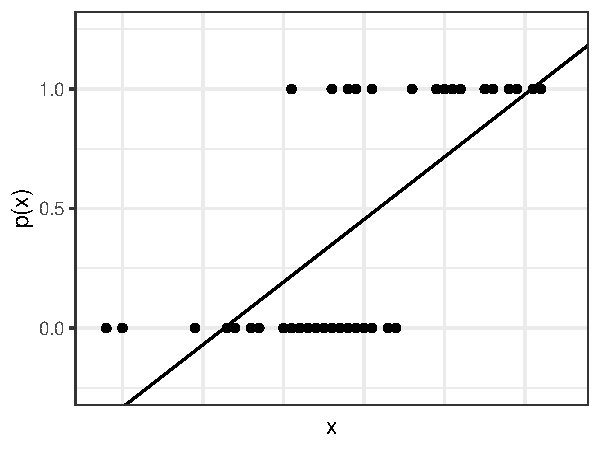
\includegraphics[scale=0.6]{figure/linreg.pdf}
\end{figure}
\end{frame}

% --------------------------------------------
\begin{frame}{Simple Logistic Regression}
Why not use linear regression to represent these probabilities?
\begin{align*}
p(x) = Pr(Y=1 | x) = \beta_0 + \beta_1 x
\end{align*}
\begin{figure}
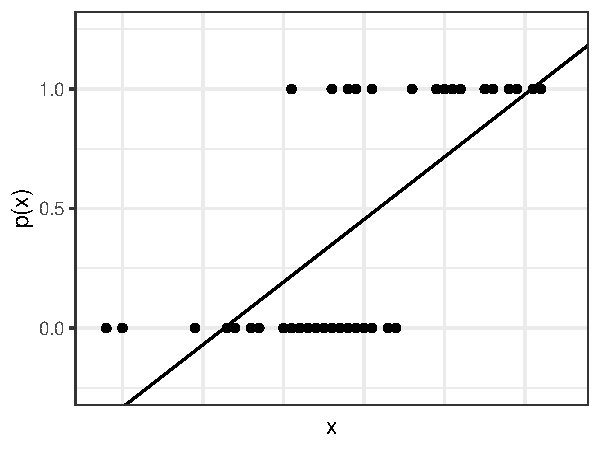
\includegraphics[scale=0.6]{figure/linreg.pdf}
\end{figure}
\textbf{Answer}:  Fitting a linear regression model can result in estimating probabilities that are less than 0 or greater than 1.
\end{frame}

% --------------------------------------------
\begin{frame}{Simple Logistic Regression}
The \textbf{logistic function} is commonly used to model $p(x)$ since it always gives outputs between 0 and 1.
\begin{align*}
p(x) = Pr(Y=1 | x) = \frac{e^{\beta_0 + \beta_1 x}}{1 + e^{\beta_0 + \beta_1 x}}
\end{align*}
\begin{figure}
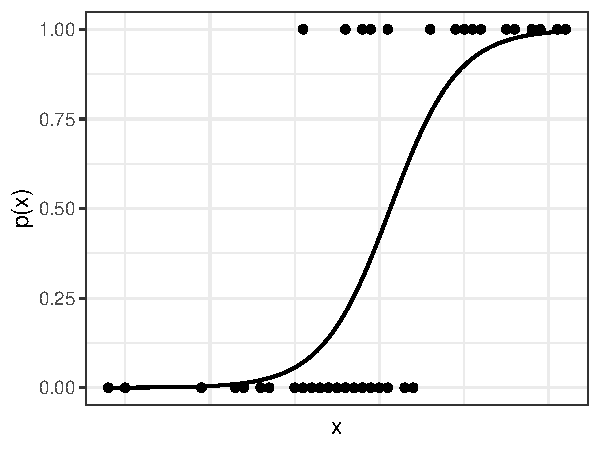
\includegraphics[scale=0.6]{figure/logistic.pdf}
\end{figure}
\end{frame}

% --------------------------------------------
\begin{frame}{Simple Logistic Regression}
Two ways to express the simple logistic regression model:\\
\vspace{10pt}

Probability form:
\begin{align*}
p(x) = Pr(Y=1 | x) 
= \frac{e^{\beta_0 + \beta_1 x}}{1 + e^{\beta_0 + \beta_1 x}}
= \frac{1}{1 + e^{-\beta_0 - \beta_1 x}}
\end{align*}
which can be interpreted as the probability $Y=1$ for a given value $x$ of the predictor.
\vspace{10pt}

Logit form:
\begin{align*}
\log\left( \frac{p(x)}{1-p(x)} \right) = \beta_0 + \beta_1 x
\end{align*}
The left-hand side is called the \emph{logit} or \emph{log-odds}.  Logistic regression expressed in terms of the logit is linear in its parameters.
\end{frame}

% --------------------------------------------
\begin{frame}{Simple Logistic Regression}
Some algebraic manipulation can be used to show that the two representations are equivalent:
\begin{align*}
p &= \frac{1}{1 + e^{-\beta_0 - \beta_1 x}}\\
\frac{1}{p} &= 1 + e^{-\beta_0 - \beta_1 x}\\
\frac{1-p}{p} &= e^{-\beta_0 - \beta_1 x}\\
\frac{p}{1-p} &= e^{\beta_0 + \beta_1 x}\\
\log\left( \frac{p}{1-p} \right) &= \beta_0 + \beta_1 x
\end{align*}
Here we are letting $p = p(x)$ to simplify notation.\\
\end{frame}

% --------------------------------------------
\begin{frame}{Inference}
Hypothesis test for $\beta_1$:\\
$H_0: \beta_1 = 0$\\
$H_A: \beta_1 \neq 0$\\
\vspace{10pt}
Test statistic:
\begin{align*}
z = \frac{\hat{\beta}_1}{se(\hat{\beta}_1)}
\end{align*}
This is sometimes referred to as the Wald z-statistic.\\
\vspace{15pt}
A $1-\alpha$ confidence interval for $\beta_1$:
\begin{align*}
\hat{\beta}_1 \pm z_{\alpha/2} se(\hat{\beta}_1)
\end{align*}
\end{frame}

% --------------------------------------------
\begin{frame}{Example: 2016 US Presidential Election}
\begin{itemize}
\item Data set called \texttt{Election16} from the \texttt{Stat2Data} library.  The data contain results from the 2016 presidential election and demographic information from all 50 states.
\vspace{10pt}
\item The binary response variable is \texttt{TrumpWin}, whether Trump won the state (1=yes, 0=no).
\vspace{10pt}
\item The predictors are
\begin{itemize}
\item \texttt{HS}: Percent of high school graduates in the state
\item \texttt{BA}: Percent of college graduates in the state
\item \texttt{Adv}: Percent with advanced degrees in the state
\item \texttt{Dem.Rep}:  Percent Democratic - Percent Republican
\item \texttt{Income}: Per capita income in the state
\end{itemize}
\end{itemize}
\end{frame}

% --------------------------------------------
\begin{frame}[fragile]{Example}
\small
\begin{verbatim}
> library(Stat2Data)
> data("Election16")
> head(Election16, n=10)
          State Abr Income   HS   BA  Adv Dem.Rep TrumpWin
1      Alabama   AL  43623 84.3 23.5  8.7     -17        1
2       Alaska   AK  72515 92.1 28.0 10.1     -17        1
3      Arizona   AZ  50255 86.0 27.5 10.2      -1        1
4     Arkansas   AR  41371 84.8 21.1  7.5      -7        1
5   California   CA  61818 81.8 31.4 11.6      16        0
6     Colorado   CO  60629 90.7 38.1 14.0      -1        0
7  Connecticut   CT  70331 89.9 37.6 16.6      11        0
8     Delaware   DE  60509 88.4 30.0 12.2       6        0
9      Florida   FL  47507 86.9 27.3  9.8       1        1
10     Georgia   GA  49620 85.4 28.8 10.7      -4        1
\end{verbatim}
\end{frame}

% --------------------------------------------
\begin{frame}[fragile]{Example}
To demonstrate simple logistic regression, we will fit a model with \texttt{TrumpWin} as the response, and \texttt{BA}, percent of college graduates in the state, as the predictor.\\
\begin{figure}
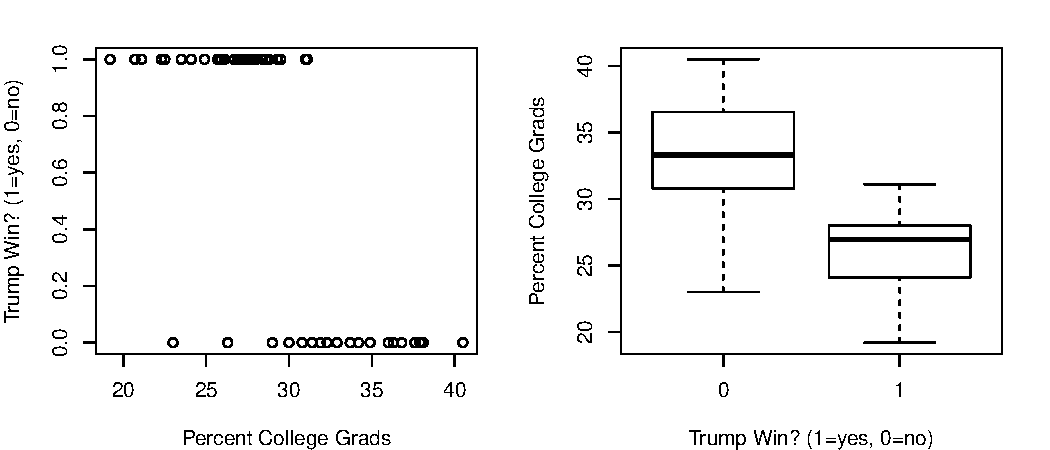
\includegraphics[scale=0.5]{figure/scatter_box.pdf}
\end{figure}
\end{frame}

% --------------------------------------------
\begin{frame}[fragile]{Example}
\small
\begin{verbatim}
> glm1 <- glm(TrumpWin ~ BA, data=Election16, family=binomial) 
> summary(glm1)

Coefficients:
            Estimate Std. Error z value Pr(>|z|)    
(Intercept)  17.9973     5.1098   3.522 0.000428 ***
BA           -0.5985     0.1735  -3.449 0.000562 ***
---
Signif. codes:  0 ‘***’ 0.001 ‘**’ 0.01 ‘*’ 0.05 ‘.’ 0.1 ‘ ’ 1

> confint(glm1)
                2.5 %     97.5 %
(Intercept)  9.809403 30.2884563
BA          -1.016162 -0.3211666
\end{verbatim}
\normalsize
\vspace{10pt}
\end{frame}

% --------------------------------------------
\begin{frame}[fragile]{Example}
\scriptsize
\begin{verbatim}
ggplot(Election16, aes(BA, TrumpWin)) + geom_point()  +
  geom_smooth(method = "glm", method.args = list(family = "binomial"), se=F) +
  xlab("Percent College Grads") + 
  ylab("Estimated Probability Trump Won") + theme_bw()
\end{verbatim}
\normalsize
\begin{figure}
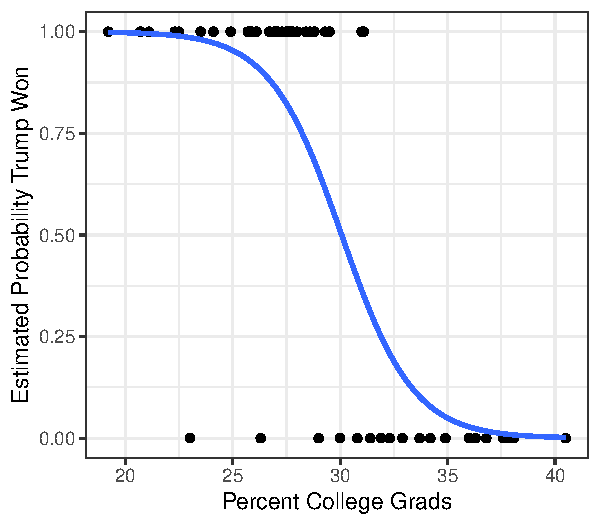
\includegraphics[scale=0.6]{figure/trump_logistic_plot1.pdf}
\end{figure}
\end{frame}

% --------------------------------------------
\begin{frame}{Example}
The fitted logistic regression model in terms of the logit:
\begin{align*}
\log\left( \frac{\hat{p}(x)}{1-\hat{p}(x)} \right) 
= \hat{\beta}_0 + \hat{\beta}_1 x
= 17.9973 - 0.5985 x
\end{align*}
\vspace{10pt}

In California, 31.4\% of the population has a BA, so the estimate for the logit is
\begin{align*}
17.9973 - 0.5985(31.4) = -0.7956
\end{align*}
\end{frame}

% --------------------------------------------
\begin{frame}{Example}
The fitted logistic regression model in probability from:
\begin{align*}
\hat{p}(x) =  \frac{e^{\hat{\beta}_0 + \hat{\beta}_1 x}}{1 + e^{\hat{\beta}_0 + \hat{\beta}_1 x}}
= \frac{e^{17.9973 - 0.5985 x}}{1 + e^{17.9973 - 0.5985 x}}
\end{align*}
\vspace{10pt}

In California, 31.4\% of the population has a BA, so the estimate for the probability that Trump won is
\begin{align*}
\hat{p}(31.4) = \frac{e^{17.9973 - 0.5985(31.4)}}{1 + e^{17.9973 - 0.5985(31.4)}}
= \frac{e^{-0.7956}}{1+e^{-0.7956}} = 0.31097
\end{align*}
\end{frame}

% --------------------------------------------
\begin{frame}[fragile]{Example}
In R, the estimate for the logit can be obtained with the command
\begin{verbatim}
> new_x <- data.frame(BA = 31.4)
> predict(glm1, newdata = new_x)
         1 
-0.7970077 
\end{verbatim}
\vspace{10pt}

The estimate for the probability can be obtained with the command
\begin{verbatim}
> new_x <- data.frame(BA = 31.4)
> predict(glm1, newdata = new_x, type="response")
       1 
0.310666 
\end{verbatim}
\vspace{10pt}

Any difference from the manual calculations are due to rounding.
\end{frame}

% --------------------------------------------
\begin{frame}{Interpreting the Coefficients}
\begin{align*}
\log\left( \frac{p(x)}{1-p(x)} \right) = \beta_0 + \beta_1 x
\end{align*}
In terms of the \emph{logit} we have the following interpretation:\\
\vspace{5pt}
An one unit increase in $x$ is associated with a change in the log-odds, or logit, by $\beta_1$.\\  
\vspace{10pt}

Going back to the example, a one unit increase in \texttt{BA} is associated with a $\hat{\beta}_1 = -0.5985$ change in the log-odds.  
\end{frame}

% --------------------------------------------
\begin{frame}{Interpreting the Coefficients}
\begin{align*}
\frac{p(x)}{1-p(x)} = e^{\beta_0 + \beta_1 x}
\end{align*}
In terms of the \emph{odds} we have the following interpretation:\\ 
\vspace{5pt}
An increase in $x$ by 1 is associated with a \emph{multiplicative} change in the odds by $e^{\beta_1}$.  In other words, a unit increase in $x$ multiplies the odds by $e^{\beta_1}$.
\vspace{10pt}

Going back to the example, a one unit increase in \texttt{BA} is associated with a multiplicative change of $e^{\hat{\beta}_1} = e^{-0.5985} = 0.55$ in the odds that Trump wins (for example, changing the odds from $4$ to $0.55(4)=2.2$).\vspace{10pt}

We can also use this interpretation for different increments.  For instance, an increase in \texttt{BA} by 0.1 is associated with a multiplicative change of $e^{0.1 (\hat{\beta_1})} = e^{0.1(-0.5985)} = 0.9419$ in the odds that Trump wins.
%Equivalently, we can say that a one unit increase in \texttt{BA} is associates with a muliplicative change of $1/e^{-0.5985} = 1.819$ in the odds that Trump lost, i.e, a 81.9\% increase in the odds that Trump lost.   
\end{frame}

% --------------------------------------------
\begin{frame}{Interpreting Coefficients}
The sign of $\beta_1$ also has meaningful interpretation:
\vspace{5pt}
\begin{itemize}
\item If $\beta_1 > 0$, then increasing $x$ will be associated with increasing the probability $p(x)$.
\vspace{5pt}
\item If $\beta_1 < 0$, then increasing $x$ will be associated with decreasing the probability $p(x)$. 
\end{itemize}
% pictures?
\end{frame}


% --------------------------------------------
\begin{frame}{Estimation}
The parameters $\beta_0$ and $\beta_1$ for logistic regression can be estimated using maximum likelihood.\\
\vspace{10pt}

Let $\{(x_i, y_i)\}$ be a sample of $n$ independent observations with $y_i \in \{0,1\}$ a binary response. Assume that $y_i$ follows a Bernoulli distribution with probability $p_i$.  We can write this compactly as:
\vspace{10pt}

$y_i \sim \text{Bern}(p_i)$\\
$Pr(y_i = 1) = p_i$\\
$Pr(y_i = 0) = 1 - p_i$\\
where $p_i$ is given by the logistic function:
\begin{align*}
p_i = \frac{e^{\beta_0 + \beta_1 x_i}}{1 + e^{\beta_0 + \beta_1 x_i}}
\end{align*}
\end{frame}

% --------------------------------------------
\begin{frame}{Estimation}
The likelihood function gives the probability of the observed zeros and ones in the data, expressed as function of the parameters. 
\begin{align*}
L(\beta_0, \beta_1) = \prod_{i=1}^n p_i^{y_i} (1-p_i)^{1-y_i}
\end{align*}
\vspace{10pt}

The log-likelihood is given by 
\begin{align*}
l(\beta_0, \beta_1) = \log(L(\beta_0, \beta_1))
= \sum_{i=1}^n [ y_i \log(p_i) + (1-y_i) \log(1-p_i)]
\end{align*}
The maximum likelihood estimates (MLEs), denoted $\hat{\beta}_0$ and $\hat{\beta}_1$, are the values of the parameters that maximize the log-likelihood function.
\end{frame}

% --------------------------------------------
\begin{frame}{Estimation}
To help understand the expression for the likelihood on the previous slide note that:
\begin{align*}
p_i^{y_i} (1-p_i)^{1-y_i} = 
\begin{cases}
p_i, &\text{ if $y_i=1$}\\ 
1-p_i, &\text{ if $y_i=0$} 
\end{cases}
\end{align*}
\end{frame}

% --------------------------------------------
\begin{frame}{Estimation}
The MLEs are computed by evaluating the partial derivatives of $l(\beta_0, \beta_1)$ with respect to each parameter and setting the equations equal to 0: 
\begin{align*}
\frac{\partial l(\beta_0, \beta_1)}{\partial \beta_0} = \sum_{i=1}^n (y_i - p_i) = 0 \qquad
\frac{\partial l(\beta_0, \beta_1)}{\partial \beta_1} = \sum_{i=1}^n x_i (y_i - p_i) = 0
\end{align*}
\begin{itemize}
\item Unlike multiple linear regression, there is no closed form for $\hat{\beta}_0$ and $\hat{\beta}_1$ that solve these equations.
\vspace{5pt}
\item Instead, iterative methods are used to solve these equations and perform the optimization. 
\vspace{5pt}
\item Popular approaches are gradient descent and the Newton-Raphson method.
\end{itemize}
\end{frame}


\end{document}
